\chapter{Introduction}
  Particle physics aims to characterize the fundamental constituents of matter and the mechanisms by which they interact. The current state of the art theory is called \emph{The Standard Model of Particle Physics} (henceforth, just the standard model), which is written in the framework of \emph{Quantum Field Theory} (QFT).

  Though the standard model has been shown to make accurate predictions in a wide range of particle physics experiments, there are no shortage of open questions as to the origin of its structure. Furthermore, the standard model does not attempt to describe gravitation, and the observation of massive neutrinos prove definitively that the standard model must be incomplete. Another observation which strongly implies a deficiency is the evidence of at least one so-called \emph{dark matter} particle, an abundant particle which does not couple to the photon with any non-trivial strength. None-the-less, it is clear that the theory which supersedes the standard model must reduce to it in the appropriate limit, and its successes should not be downplayed.

  This thesis presents the search for a dark matter candidate which couples either directly or indirectly to the Z boson. The final states studied include multiple hadronic jets, transverse momentum imbalance, and a pair of opposite-charge same-flavor leptons having dilepton mass consistent with the pole mass of the Z boson. These final states are motivated by the strengths of the CMS detector as well as simplified models of supersymmetry, a systematic framework for extending the standard model. 

\section{The standard model of particle physics}
  Nearing the turn of the 20th century, the debate on the existence of elementary particles had still not been completely settled. But in the following 80 years, a wildly rich and successful theory of matter would be developed, culminating in what is called the standard model, which has been called the best tested theory in science.

  \subsection{The evolution of particle physics} \label{sec:history}
   J.J. Thomson is credited with finding the very first elementary particle, \cite{thomson_electron} the electron. Thomson observed that cathode rays, now known to be streams of electrons, would bend under the influence of a magnetic field. This implied that rays were a beam of particles, as opposed to some sort of aether phenomena, the competing theory at the time, because they responded in accordance with the known force law for charged particles. Thomson was able to deduce the charge to mass ratio for the electrons and compared it to the known values for ionic gasses. Thomson found that the electron had a $\frac{q}{m}$ which was strikingly smaller than any ionic gas, 3 orders of magnitude smaller than hydrogen ions.

   Thomson's student, Ernest Rutherford pushed the field of particle physics further when he discovered the nucleus, and later the proton. Rutherford famously shot alpha particles (hydrogen nuclei) at a thin sheet of gold. He found that the particles mostly passed through the sheets, which implied the gold was actually a lumpy collection of heavy (when compared to the alpha particles) particles rather than a continuous material. Albert Einstein postulated the photon soon after, due to the photoelectric effect and Max Planck's famous solution to the ultraviolet catastrophe. The Neutron was discovered by James Chadwick in the 1930s after hearing about a series of experiments performed by German and French physicists found that alpha particles striking beryllium would create a penetrating radiation that was not influenced by electric fields. 

   Also in the 1930s, Hideki Yukawa used the size of the atomic nucleus to predict the existence of pions, now known to be the carriers of the strong force which counteract the repulsion of protons in the nucleus due to their charge. When looking for pions, cosmic ray experiments found muons, and mistakingly believed they had confirmed Yukawa's theory. Muons were eventually shown to not interact much with nuclei, and so they were ruled out as nuclear force carriers. Pions are produced in large numbers in the upper atmosphere, but tend to disintegrate on their way to the ground. They were eventually discovered by comic ray experiments performed in the Andes mountains.

   During the same time period, Dirac predicted the existence of antiparticles using his mathematically correct, but philosophically misguided theory of holes. The positron was discovered by Anderson when he exposed a cloud chamber to a magnetic field and discovered electron/positron pair production. Another bit of elementary particle physics uncovered during this fruitful 1930s era was that of the existence of the neutrino, which was famously theorized by Wolfgang Pauli in order to salvage energy conservation in beta decay. Enrico Fermi unified Pauli's idea with the discovery of the neutron by hypothesizing that beta decay was the decay of a neutron into a proton, an electron, and a neutrino. The electron anti-neutrino was finally discovered by observing reverse beta capture. Further observations showed muons could decay to electrons, but only in association with two neutrinos. This lead to the notion that neutrinos must carry "lepton flavor," in other words, there must be a neutrino for each lepton.

   By the 1950s, particle accelerators began to appear, and so too did the observation of a ``zoo" of new particles. These particles included some mesons which had a \emph{strangely} long lifetime, like the K$^0$, and a slew of other heavy particles. Observations suggested strange particle were always produced with another strange partner, but there was no such restriction on their decays. That fact, in addition to the long lifetime of strange particles hinted that their decays were mediated by a different force than their creation. This lead to the notion of conservation of strangeness whereby each particle was assigned a strangeness of 1, 0, or -1. Along with conservation of baryon number (theorized by Stückelberg to stabilize the proton), conservation of lepton number, and conservation of charge, a series of discrete symmetries began to appear for elementary particles. 

   Using charge and strangeness values for particles, Murray Gell-Mann developed the famous ``eightfold way," a scheme for laying out particles in geometrical patterns based on their charge and strangeness values. Arranging the particles in this way inferred the existence of a heavy particle with negative charge and -3 strangeness, now called the $\Omega^-$, which had not been observed. The observation of the $\Omega^-$ ushered in an era of particle physics which was based on symmetry principles, a trend which still dominates the field to this day.

  \begin{figure}[h!]
    \begin{picture}(150, 150)(-100, -30)
      \put(-25,42){\line(-3,-5){25}}
      \put(-25, 42){\line(1, 0){50}}
      \put(25, 42){\line(3,-5){25}}
      \put(-25, -42){\line(1,0){50}}
      \put(-25, -42){\line(-3, 5){25}}
      \put(25, -42){\line(3, 5){25}}

      \put(-25, 42){\circle*{3}}
      \put(-25, -42){\circle*{3}}
      \put(25, 42){\circle*{3}}
      \put(25, -42){\circle*{3}}
      \put(-50, 0){\circle*{3}}

      \put(50, 0){\circle*{3}}
      \put(0, 3){\circle*{3}}
      \put(0, -3){\circle*{3}}

      \put(-28, 47){$K^{0}$}
      \put(28, 47){$K^{+}$}
      \put(-28, -55){$K^{-}$}
      \put(28, -55){$\overline{K}^{0}$}
      \put(55, 0){$\pi^{+}$}
      \put(-65, 0){$\pi^{-}$}
      \put(0, 10){$\pi^{0}$}
      \put(0, -15){$\eta$}

      \put(-120, 43){$s=1$}
      \put(-120, 0){$s=0$}
      \put(-120, -43){$s=-1$}

      \put(-20, -85){$q=-1$}
      \put(45, -85){$q=0$}
      \put(70, -30){$q=1$}
    \end{picture}

    \begin{picture}(150, 150)(-375, -200)
      \put(-75,42){\line(3,-5){75}}
      \put(-75, 42){\line(1, 0){150}}
      \put(75, 42){\line(-3,-5){75}}

      \put(-25, 42){\circle*{3}}
      \put(-25, -42){\circle*{3}}
      \put(25, 42){\circle*{3}}
      \put(25, -42){\circle*{3}}
      \put(-50, 0){\circle*{3}}
      \put(50, 0){\circle*{3}}
      \put(0, 0){\circle*{3}}
      \put(0, -84){\circle*{3}}
      \put(-75, 42){\circle*{3}}
      \put(75, 42){\circle*{3}}

      \put(-78, 47){$\Delta^{-}$}
      \put(-28, 47){$\Delta^{0}$}
      \put(28, 47){$\Delta^{+}$}
      \put(78, 47){$\Delta^{++}$}
      \put(-20, -45){$\Xi^{*-}$}
      \put(30, -45){$\Xi^{*0}$}
      \put(55, 0){$\Sigma ^{*+}$}
      \put(-45, 0){$\Sigma^{*-}$}
      \put(5, 0){$\Sigma^{*0}$}
      \put(5, -84){$\Omega^{-}$}

      \put(-120, 43){$s=0$}
      \put(-120, 0){$s=-1$}
      \put(-120, -43){$s=-2$}
      \put(-120, -85){$s=-3$}

      \put(10, -120){$q=-1$}
      \put(42, -75){$q=0$}
      \put(75, -25){$q=1$}
      \put(105, 15){$q=2$}
    \end{picture}
    \vspace*{-50pt}
    \caption{The meson octet (left) and the baryon decuplet (right). Murray Gell-Mann arrayed elementary particles in these patterns and used them to predict the existence of the $\Omega^-$. This sparked a revolution in elementary particle physics based on discrete symmetries. \cite{eightfold_way}}
  \end{figure}

    Gell-Mann and Zweig independently proposed that the origin of these patterns were due to the fact that hadrons are made up of \emph{quarks}. The quark model was successful at reproducing the predictions of the eightfold way, and gave a mechanism for why particles with certain electric charges, masses, and decay pathways exist while others don't. Additionally, deep inelastic scattering experiments, much the same as Rutherford's, showed that the charge inside protons also seem to be collected in lumps, and in a way that is consistent with the three fractionally charged partons described in the quark model. \cite{proton_structure} The quark model eventually became encoded in Quantum Chromodynamics, which took it's modern form in the early 1970s with the discovery of asymptotic freedom.

    In the 1930s, the theoretical problem of infinities in quantum field theory began to emerge, specifically when calculating the mass of the electron. By the 1950s, much of the theoretical foundation for Quantum Field Theory had been laid in pursuit of a theory of Quantum Electrodynamics (QED). Julian Schwinger and Sin-itiro Tomonaga independently developed a formalism based on operator mathematics. This approach was shown to be equivalent to a formalism developed by Richard Feynman using path integrals by Freeman Dyson in 1949.\footnote{The prominant physicist Oppenheimer was so sure that Feynman's ideas were wrong that Dyson's proof earned him a lifetime appointment at the Institute for Advanced Study in Princeton without ever needing to earn a PhD.} The theoretical progress during this time explained the observation of the Lamb shift in the spectrum of hydrogen, and the electron's anomalous magnetic moment, a computation which is experimentally verified to better than 1 part per billion and has elevated the standard model to be called the best tested theory in science. In formulating the equivalence of theories, Dyson laid out criteria to decide whether a theory was renormalizable, an important feature expected from any physical QFT.

    In the 1950s an enormous theoretical breakthrough was made by Yang and Mills, who developed the concept of a Gauge theory. The gauge group SU(2)xU(1) was found to be at the heart of the unified theory of the electromagnetic and weak interactions, now called electroweak theory. Steven Weinberg invoked the Higgs mechanism in 1967 to bring the theory into modern form, showing that a massless theory in the high energy limit could "spontaneous break" into a theory with a massless photon but massive Ws and Zs at laboratory energy scales. Weinberg's theory required the existence of a scalar boson called the Higgs. \cite{Weinberg_EWK} His theory was partially confirmed with the discovery of the W and Z bosons at the UA1 and UA2 experiments at CERN in 1973. The final prediction of the electroweak theory was verified in 2012 with the discovery Higgs boson decaying to 2 photons in 2012 by the CMS and ATLAS collaborations at the Large Hadron Collider. \cite{CMS_higgs,ATLAS_higgs} The search presented in this thesis was conducted within the CMS collaboration.

    With the combination of QCD and electroweak theory, a total Lagrangian could be written with the symmetry group SU(3)xSU(2)xU(1), this is now what we called the standard model. But the particle content of the standard model still was being discovered into the next decade. In the 1970s, several breakthroughs were made. The discovery of the J/Psi meson in 1974 confirmed the existence of a fourth heavier quark, now called the charm. This brought the total number of known quarks to 4. However in the previous year experiments showed violation of CP symmetry in Kaon decays, and it was worked out by Kobayashi and Maskawa that a 4 quark model could not accommodate CP violation, at least 6 quarks were needed. 

    In 1975, the Tau lepton and it's neutrino were discovered, which gave another hint that there were 6 quarks, as it seemed natural to have the same number of quarks and leptons. Finally 1977, the bottom quark was discovered at Fermilab, giving further evidence of a sixth quark. The final piece of the puzzle was the detection of the top quark in 1995 in proton-antiproton collisions at Fermilab.

    As described above, the standard model has successfully predicted the existence of the W, Z, and Higgs bosons, including their decays. It predicted the electrons anomalous magnetic moment to extremely high precisions. It predicted the existence of a third generation of quarks and leptons based on CP violation. Indeed, at the current state of affairs, the standard model it incorporates essentially all known particle phenomenology except neutrino masses and dark matter.

\section{The Standard Model}
  The standard model of particle physics is the combination of electroweak theory with quantum chromodynamics. In section \ref{sec:history} we covered some of the highlights in the experimental and theoretical progress made while constructing this theory. In this section, we will take a look at the particle content and interactions of the standard model. 

  \begin{figure}[h!]
    \centering
    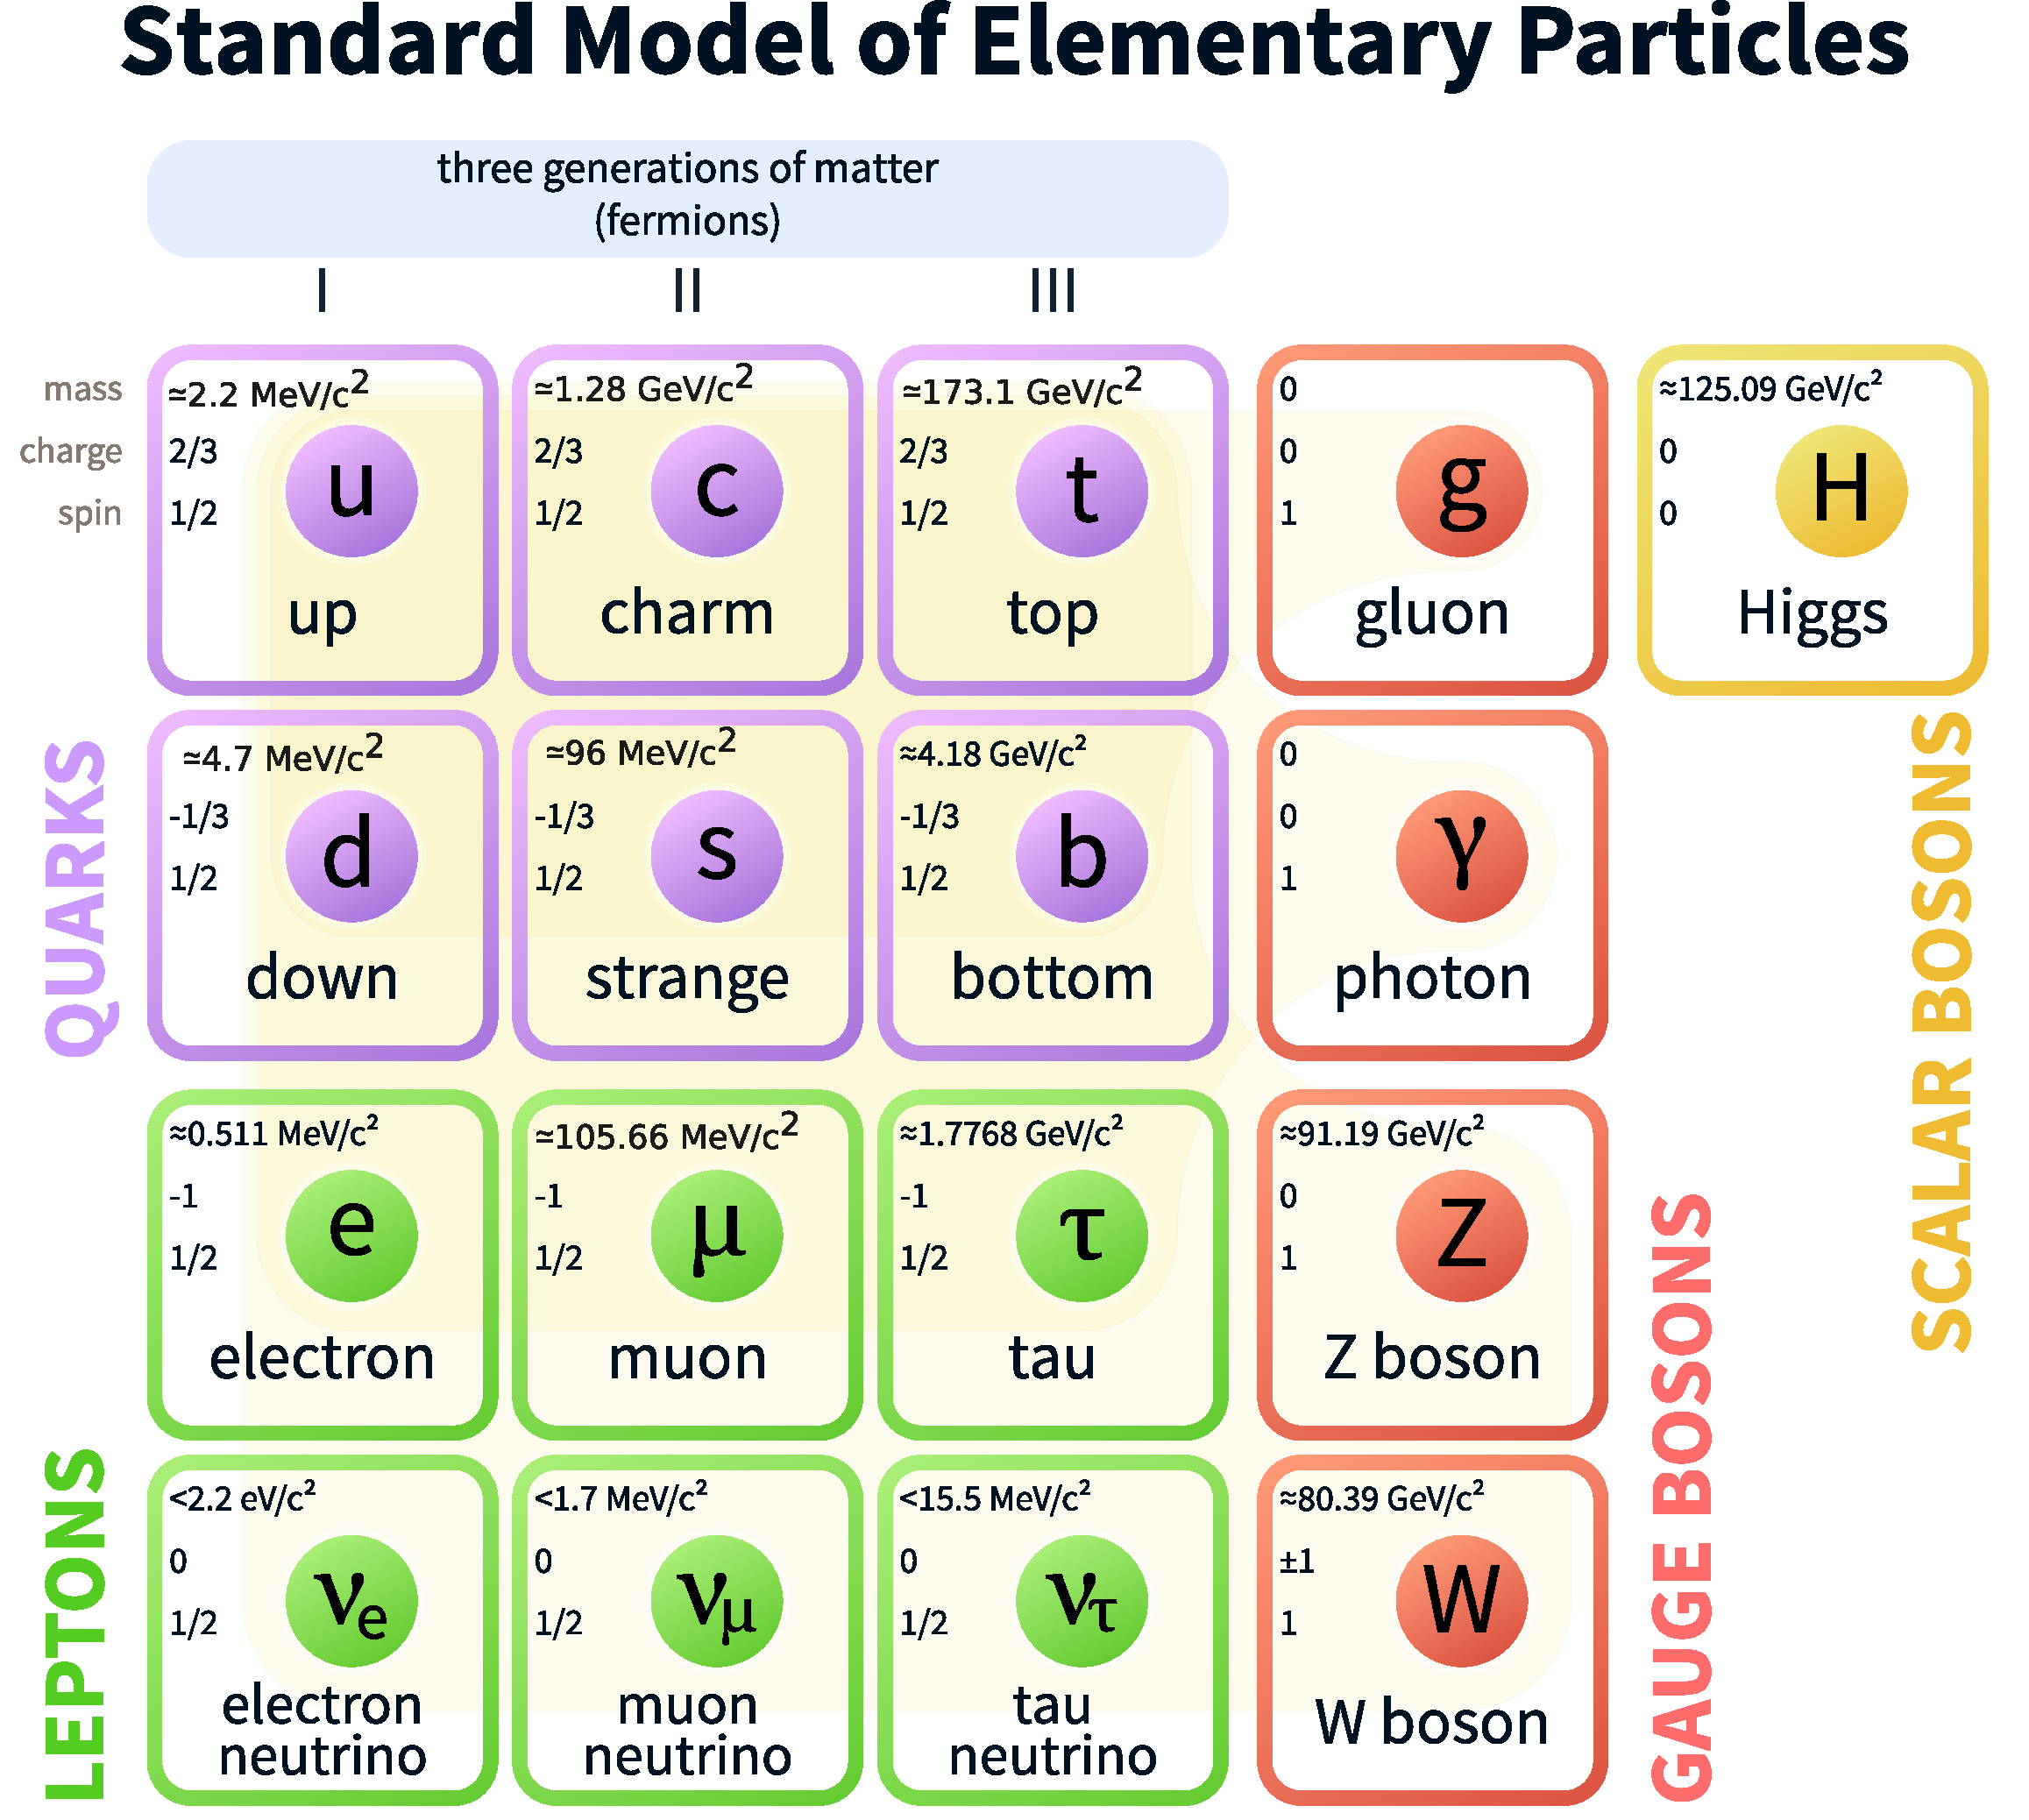
\includegraphics[width=\textwidth]{figures/standard_model_2.pdf}
    \caption{A table showing the particle content of the standard model of particle physics. Taken from \cite{SM_wiki}}
    \label{fig:standard_model}
  \end{figure}  

  Figure \ref{fig:standard_model} is a table that summarizes all the particles in the standard model. In purple, the quarks are shown. Each quark comes in one of 3 colors and has an associated anti-quark which comes in one of 3 anti-colors. In other words, the 6 slots in the figure really correspond to 36 quantum fields and equally 36 different particles. A quark is called up-type if it is positively charged (like the up quark), and down-type if it is negatively charged. The gluon comes in 8 varieties, very roughly, each gluon carries a color and an anti-color. The charged leptons: electron, muon, and tau, each come in negatively charged and positively charged varieties, positively charged leptons are called the anti-leptons. In the standard model, the neutrinos each have a partner anti-particle, but it is not known whether anti-neutrinos exist or if neutrinos are their own anti-particles. The only other hidden detail is the W boson, which comes in both positively and negatively charged variates.

  Each particle in the standard model is associated with a tensor field \footnote{A tensor a sort of generalization of a matrix, it includes real and complex numbers, vectors, matrices, and higher dimensional analogs of matrices. A tensor field associates one of these objects with each point in spacetime. For instance, a "scalar field" associates a complex number with each point in space and time. Electromagnetism associates the "Maxwell-stress tensor", a 4x4 matrix, with each point in spacetime.} that permeates all of spacetime, excitations of the fields manifest in reality as particles. The motion of particles is characterized by the propagation of excitations in spacetime. Analogously, a rock thrown into a pond will cause the water level to shift slightly downward before it breaks the surface tension. The deviation of the water height from equilibrium is a type of excitation, and it travels outward from the location the rock landed. 

  The particles in the standard model are broken up into bosons and fermions. The fermions are the quarks and the leptons, the bosons are photon, gluon, W, Z, and Higgs. The difference between bosons and fermions is characterized by their spin, which is intrinsic angular momentum a particle has even when it is at rest. Fermions have spin whose magnitude is a half integer multiple of $\hbar$, e.g. $\frac{\hbar}{2}$, $\frac{3\hbar}{2}$, etc... All standard model fermions have spin $\frac{\hbar}{2}$, typically we use units where ~$\hbar = 1$ and say standard model fermions have \emph{spin half}. Bosons have spin whose magnitude is an integer multiple of ~$\hbar$, e.g. 0, $\hbar$, $2\hbar$, etc... All the gauge bosons in the standard model have spin 1, the only boson with non unity spin is the Higgs, which has spin 0. 

  Every excitation of a quantum field takes some amount of energy. For a massive particle, the minimum amount of energy needed to make an excitation is called the mass of the particle. For instance, the minimum amount of energy needed in the muon field to make an excitation (a muon) is approximately 105 MeV. While the particle exists, this energy is trapped at the location of the particle in space. Quantum fields can exchange energy, such an event is called an \emph{interaction}. In an interaction, the energy stored in one or more quantum fields is funneled into one or more other quantum fields. For instance, a muon can decay to an electron, a muon neutrino, and an electron anti-neutrino, meaning that the energy stored in the muon was redistributed into the electron field, the muon neutrino field, and the electron anti-neutrino field.

  All interactions in QFT are local, meaning that energy can only be exchanged at roughly the same point in space and time. As an example, a muon on mars in 1970 can not create an electron and two neutrinos today in Geneva, Switzerland. Further, all interactions in the standard model are mediated by the bosons. This means a fermion can not exchange energy directly with another fermion without exchanging some energy with an appropriate boson field. In the example of the muon decaying into an electron, a muon neutrino, and an electron anti-neutrino, first the muon decays into a $W^-$ boson and a muon neutrino, then the $W^-$ boson decays into an electron and an electron anti-neutrino.

  \begin{figure}[h!]
    \centering
    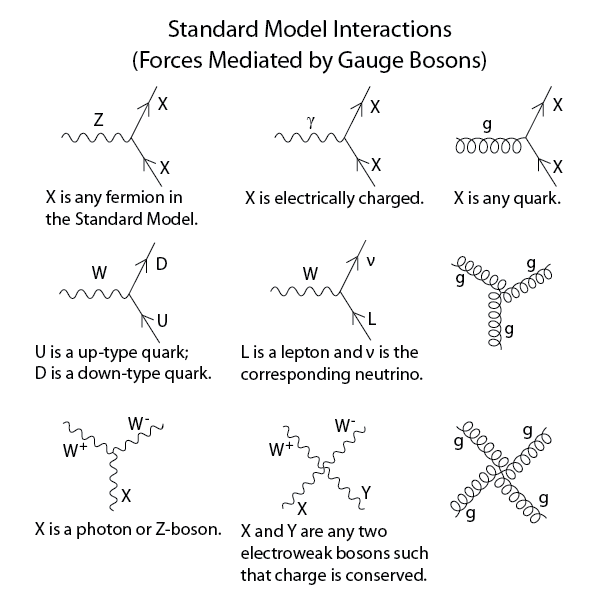
\includegraphics[width=0.7\textwidth]{figures/SM_feynman.png}
    \caption{A list of the interactions in allowed in the standard model. Taken from \cite{SM_feynman}}
    \label{fig:standard_model_feynman}
  \end{figure}  

  Figure \ref{fig:standard_model_feynman} shows the interactions allowed in the standard model. Roughly, the gluons mediate the strong interaction and can only interact with colored objects, meaning quarks and other gluons. The W and Z bosons mediate the weak interaction and can interact with any fermion as well as among themselves whilst conserving charge, with the exception of triple Z and quadruple Z interactions. The photon can interact with any charged particle.

  The rules in \ref{fig:standard_model_feynman} are called Feynman diagrams. These diagrams encode all of the discrete conservation laws in the standard model. The existence of any particle decay or production can be predicted with these rules by first checking whether these vertices can be connected together such that it turns the initial state into the desired final state, and then ensuring energy and momentum conservation will not be violated in the process.


  \subsubsection{Protons}
    The LHC is a proton-proton collider. In these collisions, the initial state particles are any particles found in protons. Figure \ref{fig:proton_pdf} shows the chance of an interaction with the different constituents of the proton in a collision, expressed as a function of the fraction of the proton's energy carried by the interacting fundamental particle.

    \begin{figure}[h!]
      \centering
      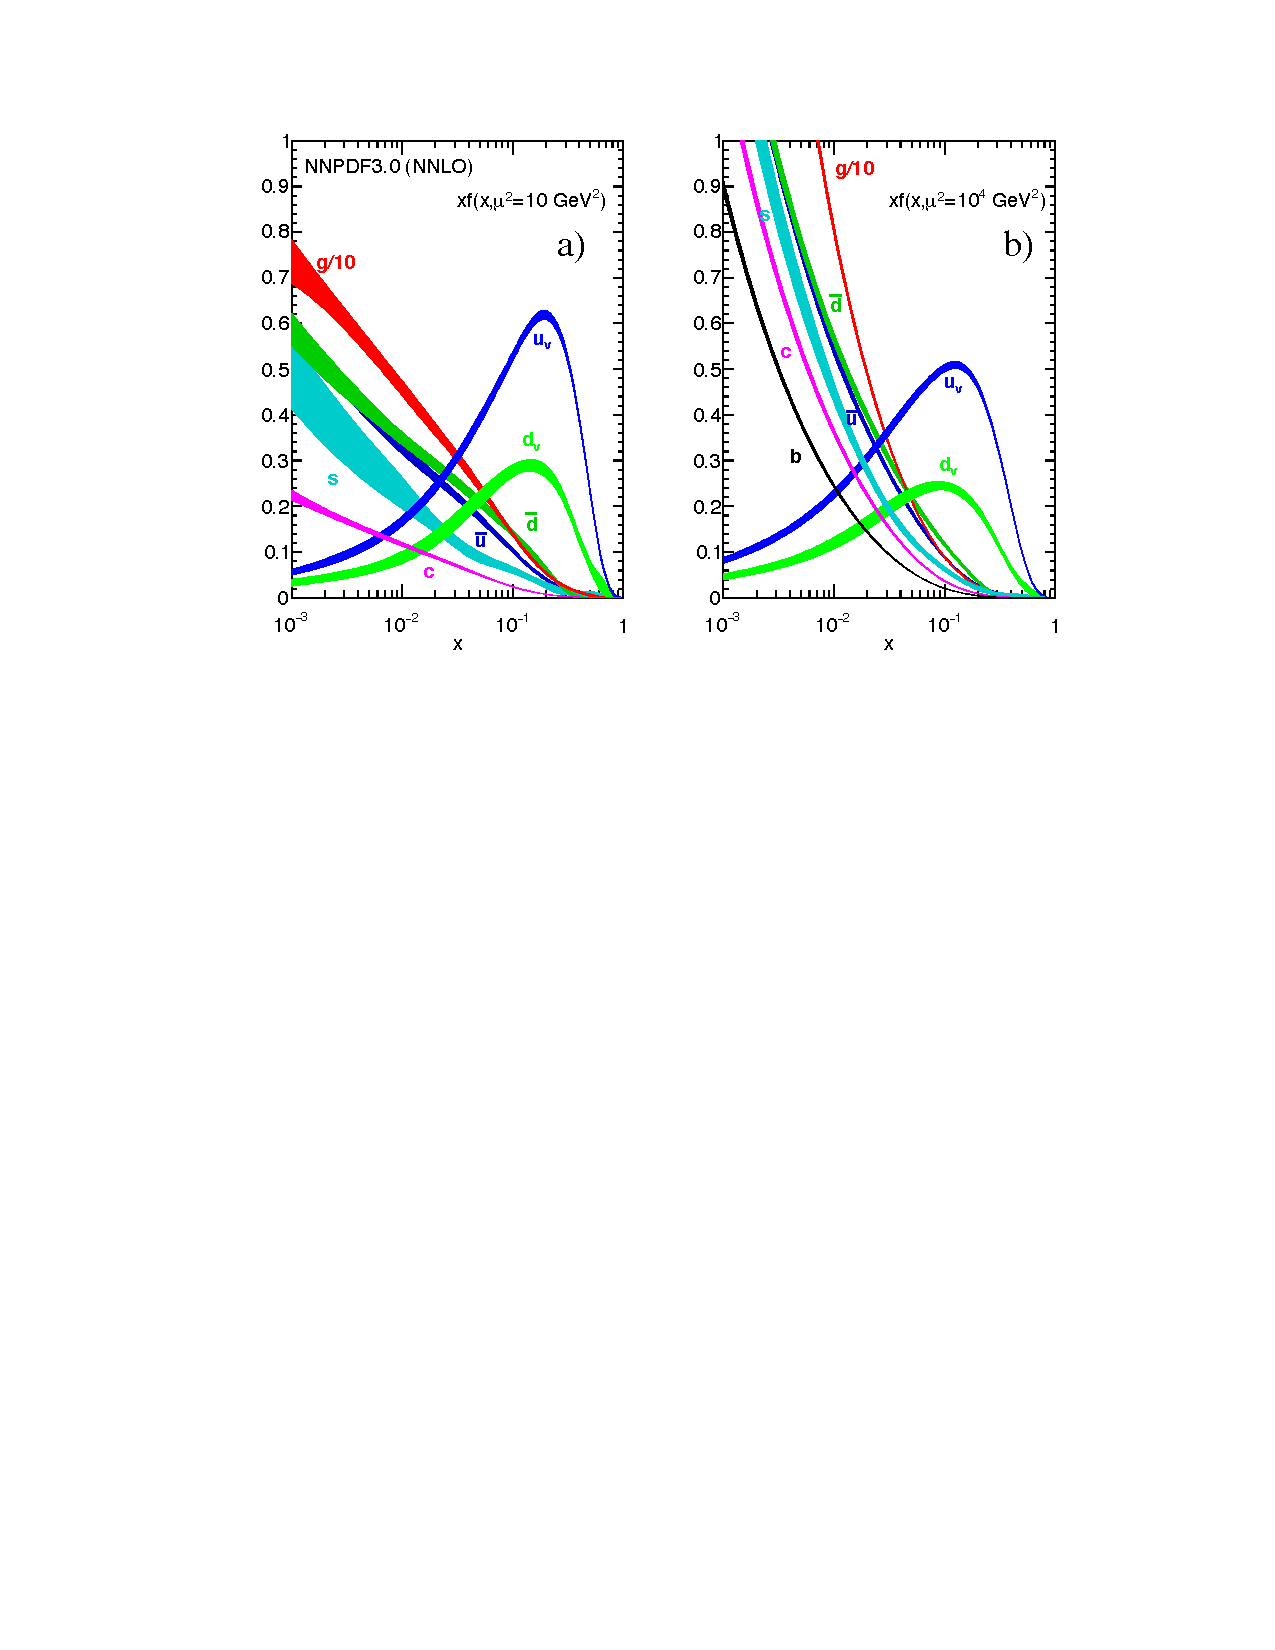
\includegraphics[width=0.7\textwidth]{figures/proton_pdf.pdf}
      \caption{The probability of colliding with a quark, by flavor, or gluon with fraction $x$ of the proton's total energy in a proton collision. The y-axis is the probability scaled by the energy fraction $x$. The gluon line has been scaled down by a factor of 10 to fit nicely with the rest of the curves, in other words, gluons are the most likely fundamental particle to interact in proton collisions. On the left (a), the curves are drawn for protons with 10 GeV of energy, on the right (b), with 100 GeV. Proton collisions at the LHC are done at approximately 7,000 GeV. The peaks for the u and d lines show the valence quark content. Taken from \cite[sec. ``Structure Functions"]{PDG}}
      \label{fig:proton_pdf}
    \end{figure}  

    Of the quarks, notice the most likely objects are the u and d quarks, in fact, there is roughly twice the chance for a u quark than a d quark. This encodes the fact that the proton is a bound QCD state of two up quarks and one down quark. However, there is still some chance to get any quark when colliding protons, this is due to the famous ``quark sea;" the energy bound up in the proton is in a superposition of particle states. One consequence of the sea for particle colliders is that the valence quark content of the particles in the collision is almost inconsequential for producing particles much lighter than the center of mass energy of the collision. 

    As a specific example, the top two entries of the left row in figure \ref{fig:standard_model_feynman} show that generating a W or Z boson from quarks requires at least one anti-quark. The naive picture of the proton as containing three quarks, uud, would predict then predict it is impossible to collide protons and produce a W or Z. However, because the W and Z are 100 times lighter than the center of mass energy of collisions, the chance of pulling an anti-up or anti-down quark from the sea with sufficient energy is large enough to compensate for the fact that there are no valiance anti-quarks. 

    In fact, the W and Z are only likely to be produced if the energy of the quarks sums to approximately 100 GeV. At large enough energies, using valence quark becomes undesirable for the production of W and Z bosons, and the cross section is dominated by sea quark seq antiquark collision. A small deviation in the W and Z cross sections between proton-proton and proton-antiproton collisions can be seen at around 2 TeV in figure \ref{fig:lhc_decay_modes}. The small dip in the cross section there reflects the change of source for the data from $p-\bar{p}$ collisions at Tevatron to $p-p$ collisions at the LHC.

\section{Problems with the Standard Model} \label{sec:problems_with_sm}
  Though the standard model has had incredible successes, there are still many open questions. The following list some observational and theoretical motivations for physics beyond the standard model. No attempt at completeness is made.

  \subsubsection{Observational Issues}

    \begin{enumerate}
      \bitem{Dark Matter} Observations in astronomy show that particle content based on the standard model can not explain the galactic rotation curves. I.e. the standard model does not contain dark matter.\cite{particle_dm}
      \bitem{Gravitation} There is no mechanism for gravitation in the standard model. Attempts to build a quantum theory of gravity using the same methods employed to build the standard model seem to fail and yield non-renormalizable theories with irreducible infinities.
      \item{Neutrino Masses} Neutrinos are modeled as massless, but neutrino oscillations show that they must have some mass.
      \item{Hubble Expansion and Inflation} There is no mechanism for dark energy, if inflation did occur, a particle called the inflaton should exist.
      \item LEP b-bbar forward backward asymmetry.
      \item anomalous muon magnetic moment.
    \end{enumerate}

  \subsubsection{Theoretical Issues}
    \begin{enumerate}
      \bitem{GUT Scale Renormalization} There is precedent to assume that at high enough energies, all three forces in the standard model combine into a single force, a Lagrangian with this feature is called a grand unified theory (GUT). The energy at which this occurs is typically called the GUT scale. Using the methods of renormalization, one can fine the GUT scale to be between $10^{15}$ and $10^{16}$ GeV. Using renormalization theory, the expected strength of the gauge interactions can be extrapolated to that energy, as can be seen in figure \ref{fig:susy_gut}. However, the standard model does not seem to show that the interaction strengths will converge at this energy. Theorists take this as a hint that the model is incomplete.
      \bitem{Naturalness and the Hierarchy problem} There are several energy scales in the standard model. The two heaviest are the electroweak scale at roughly 100 GeV and the Planck scale at roughly $10^{18}$ GeV. The electroweak scale is the mass scale of the massive electroweak bosons and the Higgs, this is where electrodynamics and the weak force combine into a single force. The Planck scale is where quantum gravitational effects are expected to become important and is the typical cutoff scale for standard model calculations. The fact that these two scales are wildly different is called the Hierarchy problem, it is also sometimes presented as the difference between the strength of gravity and the weak interaction.

      A complete exposition of theoretical aspects of the scale difference is beyond the scope of this thesis, however, the flavor of the issue is that the wildly different scales create odd interplays and ``fine-tuning" in standard model calculations. For instance, when computing the mass of the Higgs boson, the one-loop correction to the Higgs mass from a fermion $f$ is

      \[
        \Delta m_H = \frac{-\abs{\lambda_f}^2}{8 \pi^2} [\Lambda_{UV}^2 + ...]
      \]

      where $\Lambda_{UV}$ is the scale at which the theory is expected to break down, taken to be the Planck scale if no new physics exists between the standard model and quantum gravity. Therefore, the Higgs mass, measured to be 125 GeV, gets quantum corrections of order the Planck mass squared, some 30-odd orders of magnitude larger. In other words, the canonical theory requires that the sum of infinitely many terms, all of order $10^{36}$ should sum to some number which is order $10^2$ GeV.

      It is important to note that theorists disagree about the validity of this argument, as it may be reading too deeply into a perturbation calculation. However, the oddity of this calculation was one of the main driving influences behind the development of supersymmetry. As will be discussed in section \ref{sec:why_susy}, the addition of supersymmetric particles cancels the quadratic dependence on the cutoff scale in this calculation.

      \bitem{Why \emph{these} parameters} The standard model has 19 free parameters. The current theory provides no clues as to why those 19 numbers have the values they have.
      \bitem{3 Generations} Figure \ref{fig:standard_model} shows that the fermions in the SM can be grouped into three very distinct generations. The particles in these different generations are identical in all respects except for their masses. This striking feature begs for an explanation, but like the choice of parameters, the standard model has nothing to say about why three generations of fermions exist.
      \bitem{Strong CP Problem} A discrete symmetry of the standard model is called CP. An interaction obeying CP symmetry implies that anti-particles which spin in some direction should experience the same interactions with the same strengths as regular particles which spin the opposite direction. Why does QCD respect CP symmetry while it is essentially maximally broken in the electroweak theory?
      \bitem{unstable universe} The universe is said to be in a metastable state given the standard model fits. Taken at face value, this means the Higgs field could decay at any moment and destroy the universe. Like Schrodinger's cat, the absurdity of this result can be considered motivation for a theory which gives less ridiculous predictions.
    \end{enumerate}                 
  
\section{The Solutions of Supersymmetry}
  Supersymmetry (SUSY) is a framework which can be used to build infinitely many extensions of the SM. It can be traced back to the late 1960s, with the first physical models of SUSY in 4 dimensions discovered by Weiss and Zumio in the 1974. \cite[ch. 24]{weinberg_SUSY} The key idea behind SUSY is the treatment of boson and fermion fields as pairs, called \emph{superpartners}.\footnote{The most commonly cited review is \cite{susy_primer}} A Lagrangian is called supersymmetric, roughly, if you can interchange the two superpartners without changing its physical predictions. It illustrates the right flavor to say ``the superpartners experience the same interactions."\footnote{This is an overstatement. In reality, supersymmetry transformations are built through infinitesimal translations of the fields which depend on the superpartner's state. Fields and their superpartners will be mathematical objects with different dimensions, a strict substitution doesn't truly make sense. \todo{Is this right?}}

  It is useful now to introduce some terminology. Particles which appear in the standard model are called \emph{baryonic matter}\footnote{This is a bit of a misnomer given leptons and the gauge bosons carry no baryon number, but are still lumped into this classification}. Superpartners to baryonic matter are called \emph{sparticles}, a portmanteau of supersymmetric and particles. The superpartners of quarks and leptons are called squarks and sleptons respectively; here the ``s" stands for scalar. For technical reasons based on the chiral nature of some standard model interaction, superpartners of fermions must have spin 0. Finally, the superpartners of the gauge bosons are given the suffix -ino, e.g. gluino and Zino, they are collectively called the gauginos. 

  \subsection{The Minimal Supersymmetric Standard Model Extension}
    Supersymmetry operators take bosons into fermions and visa versa. It is possible to construct SUSY theories where each standard model particle has multiple superpartners, typically the number of superpartners in a SUSY theory is denoted by $\EuScript{N}$. The minimal model of SUSY that incorporates the standard model has one superpartner, $\EuScript{N} = 1$, and is called the Minimal Supersymmetric Standard Model (MSSM). 

    The particle content of the MSSM is not precisely double the particle content of the standard model. For technical reasons, the number of Higgs-like bosons in the MSSM is expected to be 5 in total. These include the known Higgs, being the lightest at 125 GeV, two charged Higgs called the H$^+$ and H$-$, and two neutral Higgs called the A and H. In addition, gravitation can be incorporated into SUSY theories. The $\EuScript{N} = 1$ SUSY theory with gravitation is called the minimal supersymmetric theory of gravity (mSUGRA). These theories include massless gravitons and their superpartner, gravitinos. 

  \subsection{R-parity} \label{sec:r-parity}

    An attractive ad-hoc symmetry is added is to most supersymmetry models called R-parity. R-parity requires a multiplicatively conserved quantum number at each interaction vertex. Each particle is assigned a number

    \[
      P_R = (-1)^{3(B-L)+2s}.
    \]

    $P_R = +1$ for baryonic matter and $P_R = -1$ for sparticles. Without R-parity, SUSY models would allow for the violation of baryon and lepton numbers in laboratory decays, while no such decays have ever been detected. A particularly strong limit on R-parity violation comes from the proton lifetime, which is currently observed as $> 10^{32}$ years, 22 orders of magnitude larger than the age of the universe. 

    Another consequence of exact R-parity conservation is that there must be an even number of sparticles at each interaction vertex. With baryonic initial states, like at the LHC, SUSY particles would need to be pair produced. Additionally, heavy sparticle decay products must include at least one lighter sparticle. Taking this to its logical conclusion, the lightest supersymmetric particle (LSP) will be absolutely stable, i.e. will not be able to decay into standard model particles even if they are lighter, and must eventually appear as part of the decay chain of any SUSY particle produced. This means that in models with R-parity conservation, the LSP could provide a ubiquitous dark matter candidate, provided it is electrically neutral. \cite[sec. 6.2]{susy_primer}

  \subsection{SUSY Breaking}
    If supersymmetry were an exact symmetry, then sparticles should have the same mass as their standard model superpartner. For instance, a selectron should exist with a mass of 0.511 MeV, such a particle should have been produced in laboratory experiments long ago. Because no such sparticles have been observed, there must be a breaking of SUSY in the vacuum state of that we experience as our physical reality. Such a phenomena is known as spontaneous symmetry breaking, a short review can be found in \cite{symmetry_breaking}. Theoretical investigations show that in most scenarios for SUSY breaking, the sparticles are expected to have their own mass scale and not vary in mass over more than an order of magnitude. This is an important feature because the non-observation of sparticles implies they are heavier than baryonic matter. 

    Another important feature of SUSY breaking is the possibility of mixing of electroweak gaugino and higgsino states, as well as inter-squark mixing and inter-slepton mixing. This means that the mass eigenstates seen in nature do not need to correspond to the SUSY eigenstates. As an example, if SUSY exists in nature, a collider like the LHC need not produce exactly selectrons or smuons, but rather particles which are some linear combination of those states.

    The scale of SUSY breaking is related to its attractiveness as an extension to the standard model. The hierarchy problem can be boiled down to a sensitivity of the low energy physics in the standard model to physics at arbitrarily high energy scales. Put very roughly, SUSY is the fix for this problem given that the superpartner masses are not large compared to the Planck mass.\cite[pg. 11]{susy_primer} Using this criteria, SUSY breaking models estimate that the mass scale of SUSY particles should not be much larger than a few TeV. This is sometimes called ``electroweak scale SUSY breaking," and it is main reason many scientists at CERN are looking at SUSY models to motivate searches for new particles.

    Theoretical investigations of SUSY breaking show that it is not possible to accommodate SUSY breaking scenarios where all standard model particle masses are lighter than their superpartners without invoking a so-called ``hidden sector", a group of particles which do not interact strongly with the standard model particles or their superpartners with large couplings. One class of these models is called gauge mediated SUSY breaking (GMSB), a schematic of which is shown in figure \ref{fig:gmsb}. In GMSB, SUSY is broken in the hidden sector, which couples to another auxiliary messenger sector. The messenger sector then can be coupled to the MSSM by normal SU(3)$_C \times $ SU(2)$_L \times $ U(1)$_Y $ gauge and gaugino interactions.\cite{gmsb}

    \begin{figure}[h!]
      \centering
      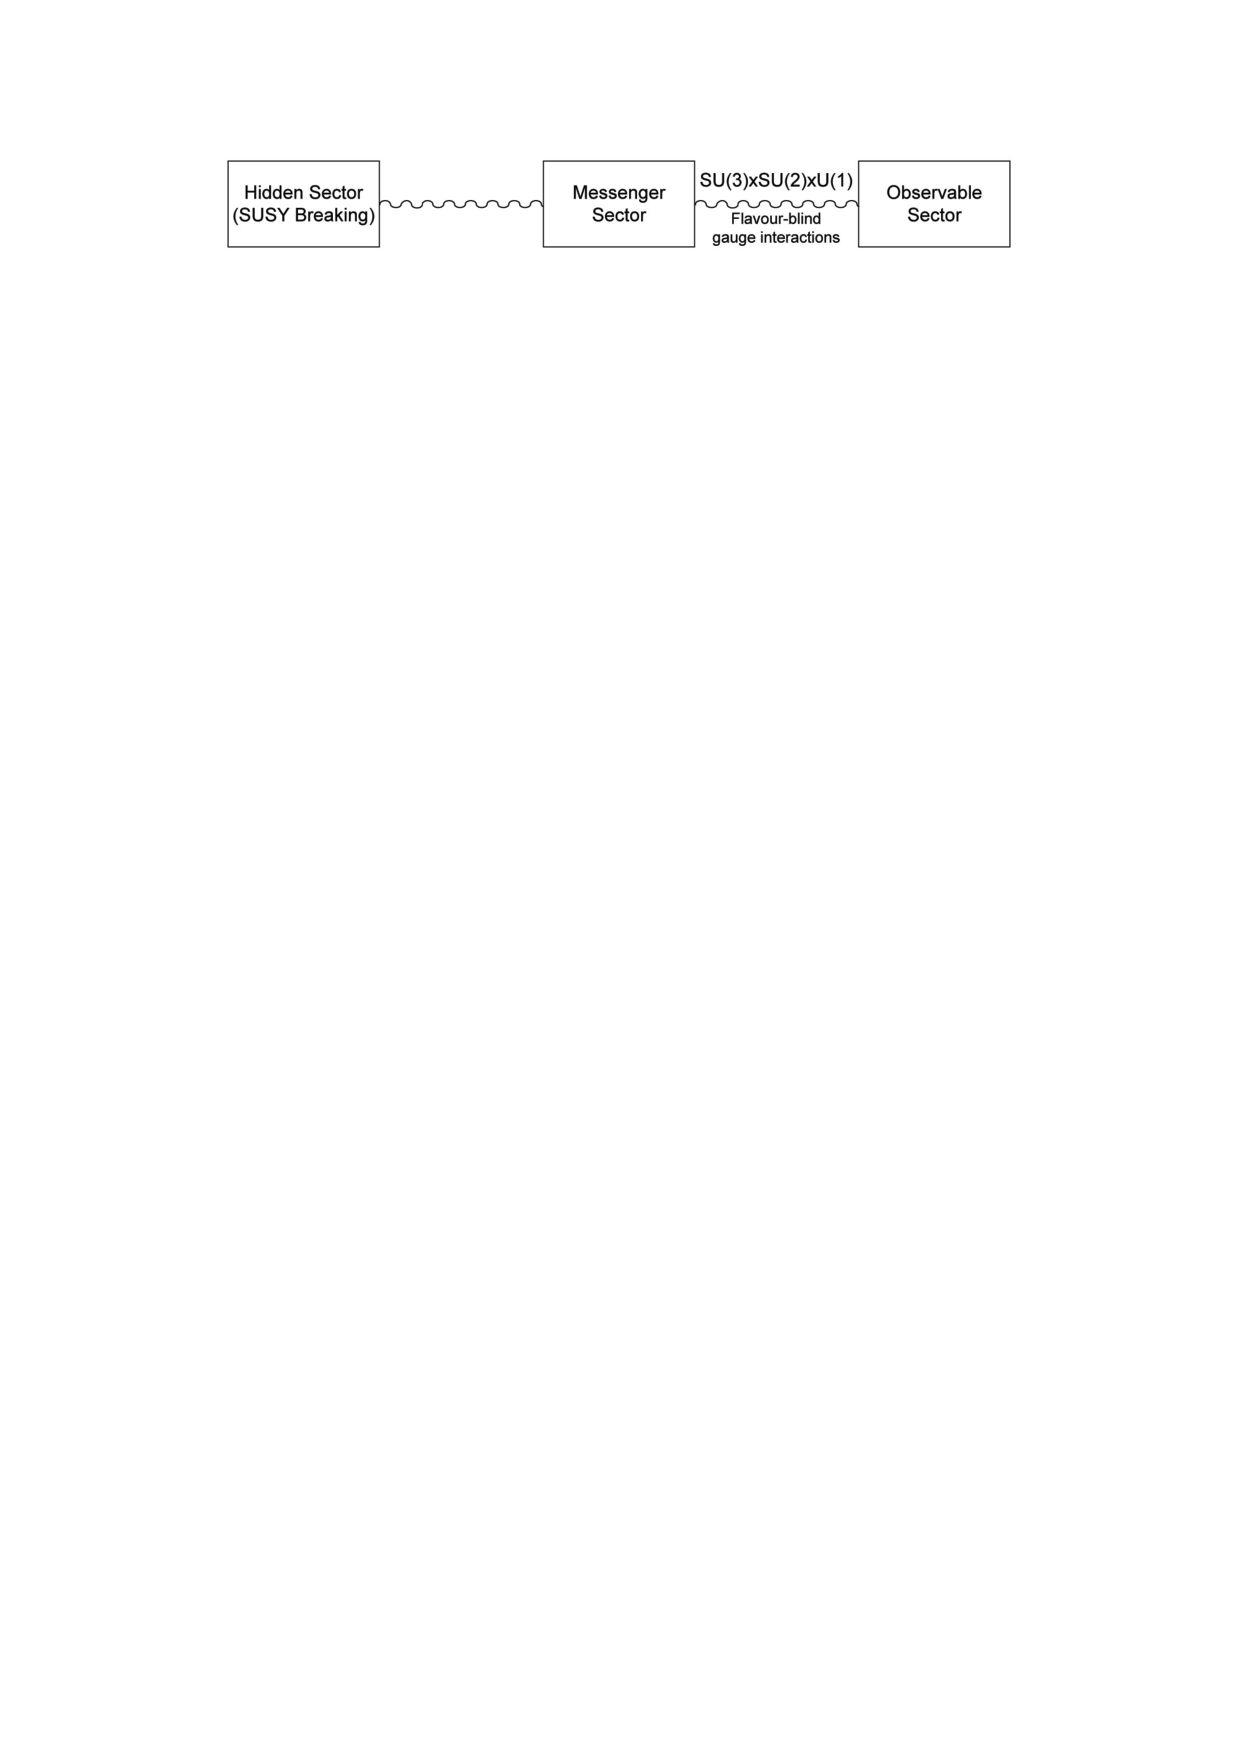
\includegraphics[width=\textwidth]{figures/gmsb.pdf}
      \caption{A schematic diagram showing the structure of GMSB models. A hidden sector exists which is the source of SUSY breaking. The hidden sector interacts with a messenger sector, which in turn has interactions with the MSSM particles in a ``flavor blind way". Taken from \cite{gmsb}}
      \label{fig:gmsb}
    \end{figure}

  \subsection{Simplified Models}
    The MSSM itself adds over 100 free parameters to the standard model, not including those that come from the SUSY breaking scheme or gravitation. The large parameter space dimensionality of realistic SUSY models make them extremely difficult to compare with observation. In order to address this issue, a series simplified models of supersymmetry have been developed which attempt to target specific phenomenology of the MSSM. In these models, 

  \subsection{Why SUSY?}
    Above, we gave a very brief introduction to SUSY and touched on some features of SUSY theories that make it attractive to study. Below, we attempt to summarize the main motivations for distinguishing SUSY as an extension to the standard model.

    \begin{itemize}
    \item Supersymmetry offers a solution to the hierarchy problem described in section \ref{sec:problems_with_sm} by automatically including exactly canceling counter-terms for the large quantum corrections to scalar particle masses, like the Higgs mass.
    \item One of the issues with supersymmetry is that SUSY models typically predict proton decay. In order to stop proton decay, a new symmetry called R-parity is imposed, and most physical models of SUSY assume R-parity holds. In models with R-parity conservation, supersymmetry provides a natural dark matter candidate. The lightest supersymmetric particle (LSP) should not be able to decay to regular matter because of the new conservation law, and so an electrically neutral LSP could be the dark matter we see in astrophysical observations.
    \item The minimal supersymmetric extension to the standard model, i.e. the addition of one superpartner for each SM particle, seems to be able to accommodate a GUT Lagrangian, as shown in figure \ref{fig:susy_gut}.
    \item Though not mentioned specifically in the previous discussion, some of the interest in SUSY comes from mathematical considerations. Mathematically, supersymmetry is the only known caveat to the Coleman-Mandula theorem, which states that the symmetry group of non-trivial QFTs must be written as
      \[
      G_{\text{Poincaré}} \times G_{\text{internal}}.
      \]
      This result is known as the Haag–Łopuszański–Sohnius theorem. Broadly speaking, supersymmetry is the only known caveat to a quite strong restriction on the structure of QFTs.
    \end{itemize}

    \begin{figure}[h!]
      \centering
      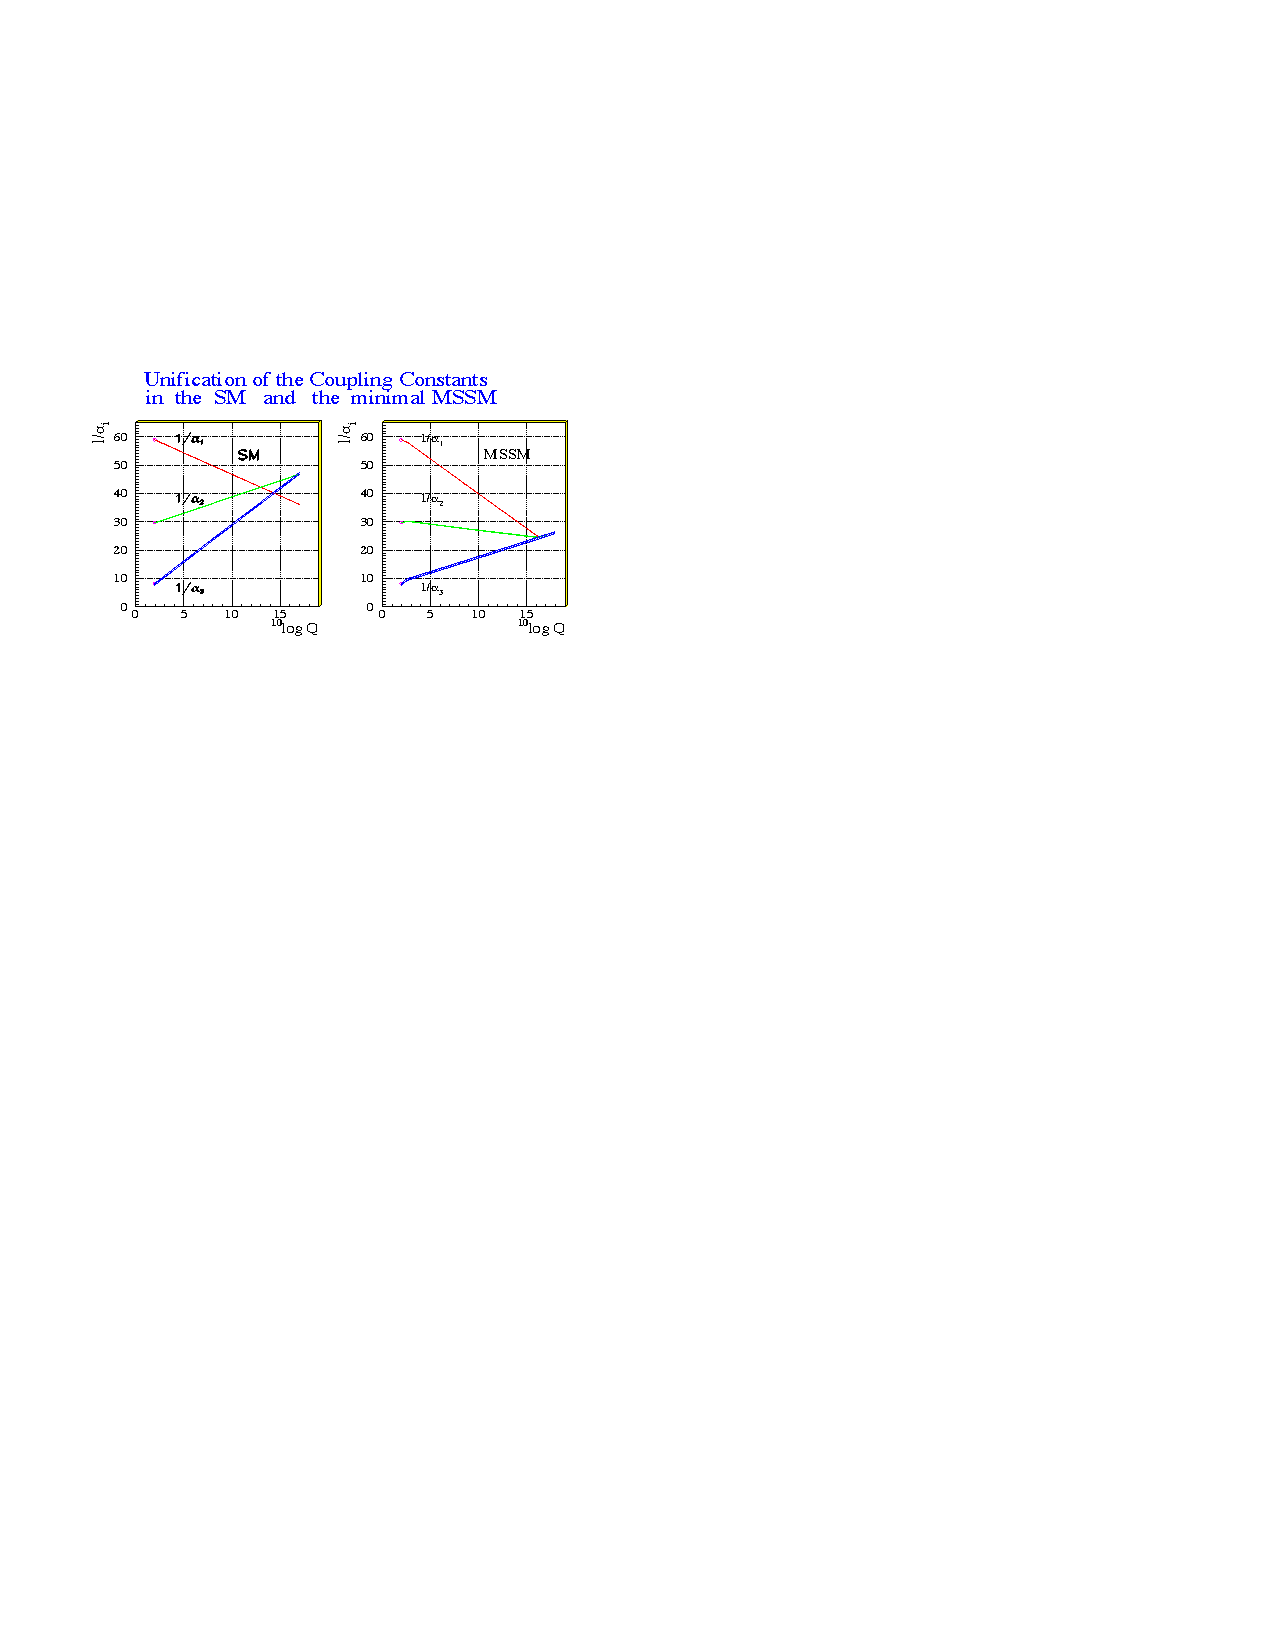
\includegraphics[width=.7\textwidth]{figures/SUSY_GUT_couplings.pdf}
      \caption{The strength of the strong[SU(3)] and electroweak [SU(2)xU(1)] coupling constants. On the left, the prediction derived from the standard model is shown, and the right the predictions from the MSSM. In a grand unified theory, the lines are expected to meet at a single point where all the forces unite and therefore have equal strength. There are 8 standard deviations separating a perfect fit for the standard model (i.e. assuming no new particles heavier than the top quark exist), while the MSSM accommodates a unification point much more readily. This is interpreted as a sign that the MSSM might be the legitimate GUT of nature. Taken from \cite{SUSY_RG}}
      \label{fig:susy_gut}
    \end{figure}
    
\section{Why focus on the Z with \MET final state?}
  As mentioned in the introduction, the ZMET final state is motivated partially by considerations about the detector and partially by simplified supersymmetric models. Leptons at the LHC are rarely produced compared to hadronic jets,\ref{sec:what_gets_made} and are typically measured with high energy resolution (\ref{sec:electron_measurement_pipeline}, \ref{sec:muon_measurement_pipeline}). This makes a leptonically decaying Z boson a great object to tag as the energy resolution of the Z will be good and the standard model backgrounds for opposite-charge same-flavor leptons with dilepton mass near the Z pole mass is extremely low. The main production method of Z bosons in proton-proton collisions is Drell-Yan production. To reduce this background, we require at least 2 jets are 

  \subsection{Past results}
  An analysis in this final state has been published several times from the CMS collaboration, with the latest iteration in 2016.\cite{paper_2012, paper_2015, paper_2016} The differences between the previous version and the analysis presented in this thesis are summarized below:
  \begin{itemize}
    \item The integrated luminosity analyzed increased by a factor of 15.
    \item Search regions were added to target SUSY production leading to final states contain an additional W or Z boson (VZ), and final states containing a Higgs boson (HZ). Interpretations in simplified models that produce these final states were also added. \ref{sec:search_regions}
    \item A correction is now applied to the photon sample used in the Z+Hadronic background prediction to subtract away events with real \MET. \ref{sec:ewk_subtraction}
    \item A new method for the flavor symmetric background prediction was developed which uses same-sign events outside the Z mass window to predict the MET spectrum inside. \ref{sec:kappa}
  \end{itemize}